\documentclass[11pt]{article}

\usepackage[utf8]{inputenc}
\usepackage[T1]{fontenc}
\usepackage[margin=1in]{geometry}
\usepackage{algorithm}
\usepackage{algpseudocode}
\usepackage{tikz}
\usepackage{amsmath, amssymb}
\usepackage{float}
\usetikzlibrary{trees}

\bibliographystyle{plain}


\title{TODO Add a name}
\author{Kevin Chen}
\date{\today}

\begin{document}

\maketitle

\section{Introduction}

TODO insert introduction

\section{Symbolic Execution}

Symbolic execution is a way of executing a program abstractly, such that on abstract execution covers multiple possible inputs of the program that share a particular execution path through the code \cite{aldrich2018symbolic}. Each input of symbolicly executed code is represented as a symbol rather than assigning it a concrete value. When the value is referenced such as for an if statement, the execution path branches, where one path the symbolic value is evaluated as true while the other path the symboilic value is evaluated as false.

One of the key uses for symbolic execution is in testing. Most unit tests, require the programmer to hardcode in values to test, resulting in various unit tests to cover all branches the code can tranverse. On the other hand, a symbolic execution would execute simutaneously on a family of inputs. Consider the following example:

\begin{algorithm}
    \caption{Algorithm 1}
    \label{alg:simple-example}
    \begin{algorithmic}[1]
    \Require $x, y \in \mathbb{Z}$
    \State $a \gets x + y$
    \If{$a \bmod 2 = 0$}
        \State \Return error ``$a$ is even''
    \Else
        \State \Return $a$
    \EndIf
    \end{algorithmic}
\end{algorithm}
    
With a glance, we can see that using any combination of numbers such that their sum results in an even number will result in an error. There is no way to cover all cases of failure using unit tests, as there are an infinite number of way which we can stumble onto this error.

Instead of testing with unit tests such as $x=1, y=1$, symbolic execution represents the inputs as symbols $x=x_0, y= y_0$. Whenever, the symbols are required to return a value, such as in a branch, symbolic execution splits into two executions, with each execution recording the branching condition in its execution path. Consider a symbolic execution of the algorithm above. We start with representing each input symbolicly:

\begin{figure}[H]
    \centering
    \begin{tabular}{|c|c|c|}
        \hline
        line & Path Condition & Translation \\
        \hline
        0 & true & $x\to x_0, y\to y_0$ \\
        1 & true & $x\to x_0, y\to y_0, a\to x_0+y_0$ \\
        2 & $(x_0 + y_0) \bmod 2 = 0$ & $x\to x_0, y\to y_0, a\to x_0+y_0$ \\
        2 & $\neg((x_0 + y_0) \bmod 2 = 0)$ & $x\to x_0, y\to y_0, a\to x_0+y_0$ \\
        3 & $(x_0 + y_0) \bmod 2 = 0$ & Error \\
        5 & $\neg((x_0 + y_0) \bmod 2 = 0)$ & Return $x_0 + y_0$ \\
        \hline
    \end{tabular}
    \caption{Symbolic execution trace showing path conditions and variable translations}
    \label{fig:symbolic-trace}
\end{figure}

In this example, we see that the inputs values start symbolic as symbols which has no concrete value. Following the execution, we translate every instance of $x$ with $x_0$ with the same case for $y$. Where it gets interesting is when the the execution has a branching path. In the $\textbf{if}$ statement, the value of a is required to be assigned a value, which breaks the symbolic abstraction. Instead, the symbolic execution branches into two different executions, each of which assuming a different condition to satisfy the branching statement. Below we can visualize the different execution paths the execution takes via a simple tree (see Figure~\ref{fig:execution-tree}):

\begin{figure}[H]
    \centering
    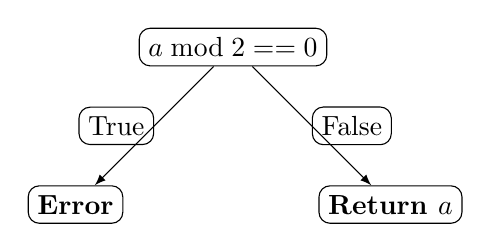
\begin{tikzpicture}[
        level distance=2cm,
        sibling distance=4cm,
        every node/.style={draw, rounded corners, align=center},
        edge from parent/.style={draw, -latex}
      ]
      
      \node {$a \bmod 2 == 0$}
          child { node {\textbf{Error}}
              edge from parent node[left] {True}
          }
          child { node {\textbf{Return $a$}}
              edge from parent node[right] {False}
          };
      
      \end{tikzpicture}
    \caption{Execution tree showing the branching paths in symbolic execution}
    \label{fig:execution-tree}
\end{figure}

In each paths, we accumulate the different path conditions until we either reach the end (return statement) or a failure (error). In this case, we find that there exists a set of inputs (when $x_0+y_0 \bmod 2 = 0$), which causes an error. Now imagine a different example; using the same coding example, but with a twist. Prior to running this program with symbolic execution, one can add constraints to the path. Below, an example where we start with a given constraint that $x_0+y_0=1$:

\begin{figure}[H]
    \centering
    \begin{tabular}{|c|c|c|}
        \hline
        line & Path Condition & Translation \\
        \hline
        0 & $x_0+y_0=1$ & $x\to x_0, y\to y_0$ \\
        1 & $x_0+y_0=1$ & $x\to x_0, y\to y_0, a\to x_0+y_0$ \\
        2 & $\neg((x_0 + y_0) \bmod 2 = 0)$ & $x\to x_0, y\to y_0, a\to x_0+y_0$ \\
        2 &  $x_0+y_0=1 \land (x_0 + y_0) \bmod 2 = 0$ & $x\to x_0, y\to y_0, a\to x_0+y_0$ \\
        3 & False & Error \\
        5 & $\neg((x_0 + y_0) \bmod 2 = 0)$ & Return $x_0 + y_0$ \\
        \hline
    \end{tabular}
    \caption{Modified version of execution with existing constraints}
    \label{fig:symbolic-trace-with-constraint}
\end{figure}

With the constraint, the path condition which leads to the error is contradictory. This illustrates that the path is impossible. With this constraint, we see that no path leads to any errors. In industry, programmers, can create tests with given preconditions (constraints) and run until the program terminates. Instead of throwing an error, we can use assertion statements as post-conditions. If it terminates without an error, the program is robust across all set of inputs. Otherwise, a symbolicly executed program will return a concrete set of conditions which will give an error or violate a post-condtiion.

\subsection{While loops}

To represent a while loop in symbolic execution, we unroll it into a recursive function with no loops. Take the following code for instance:

\begin{algorithm}
    \caption{Count Number of 1's in a Bit Vector}
    \label{alg:count-ones-while}
    \begin{algorithmic}[1]
    \Require $v$ is a bit vector of length $n$
    \State $count \gets 0$
    \State $i \gets 0$
    \While{$i < n$}
        \If{$v[i] == 1$}
            \State $count \gets count + 1$
        \EndIf
        \State $i \gets i + 1$
    \EndWhile
    \State \Return $count$
    \end{algorithmic}
\end{algorithm}

We can rewrite it as a recursive function: 

\begin{algorithm}
    \caption{Recursively Count Number of 1's in a Bit Vector}
    \label{alg:recursive-count-ones}
    \begin{algorithmic}[1]
    \Require $v$ is a bit vector of length $n$
    \Function{count\_ones}{$v, i, n$}
        \If{$i == n$}
            \State \Return $0$
        \ElsIf{$v[i] == 1$}
            \State \Return $1 +$ \Call{count\_ones}{$v, i+1, n$}
        \Else
            \State \Return \Call{count\_ones}{$v, i+1, n$}
        \EndIf
    \EndFunction
    \State \Return \Call{count\_ones}{$v, 0, n$}
    \end{algorithmic}
\end{algorithm}

Now that we have rewritten the while loop as if statements, we simply create a new branch for every if statement. In practice, this may lead to state explosion, resulting in thousands of branches in a just a few iterations. Programmers either set a recursion limit, terminating the branch which gets stuck, or find a different way to represent the while loop, using the loop invariant. Below is a tree of the branching paths created from a symbolic execution of Algorithm~\ref{alg:recursive-count-ones}. 

\begin{figure}[H]
    \centering
    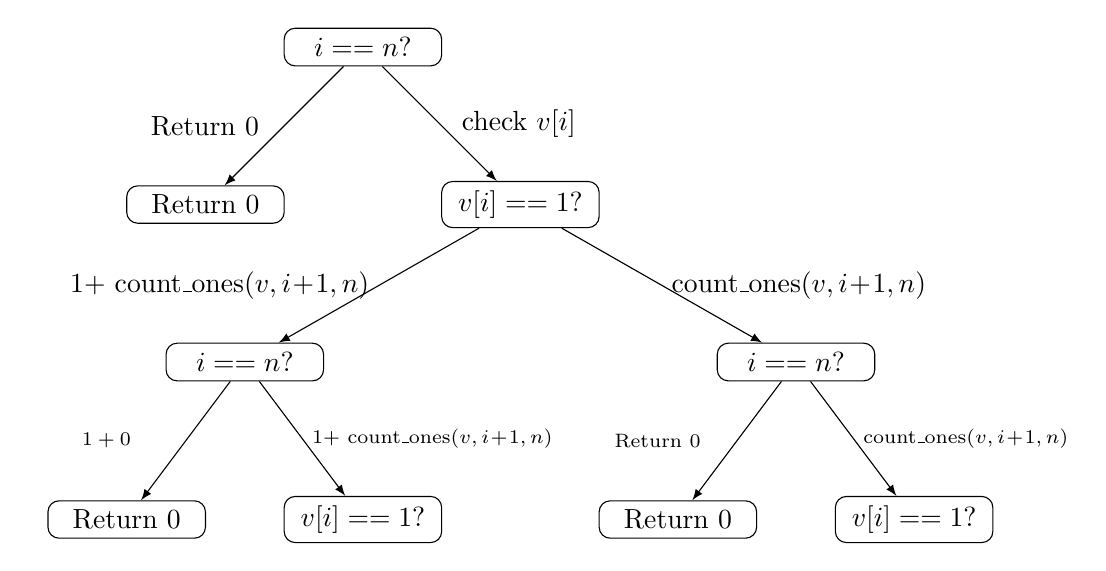
\begin{tikzpicture}[
        level 1/.style={sibling distance=4cm, level distance=2cm},
        level 2/.style={sibling distance=7cm, level distance=2cm},
        level 3/.style={sibling distance=3cm, level distance=2cm},
        every node/.style={draw, rounded corners, align=center, minimum width=2cm},
        edge from parent/.style={draw, -latex}
      ]
      
      \node {$i == n$?}
          child { node {Return 0}
              edge from parent node[left, draw=none] {Return 0}
          }
          child { node {$v[i] == 1$?}
              child { node {$i == n$?}
                  child { node {Return 0}
                      edge from parent node[left, draw=none, font=\scriptsize] {$1 + 0$}
                  }
                  child { node {$v[i] == 1$?}
                      edge from parent node[right, draw=none, font=\scriptsize] {$1 +$ count\_ones($v, i\!+\!1, n$)}
                  }
                  edge from parent node[left, draw=none] {$1 +$ count\_ones($v, i\!+\!1, n$)}
              }
              child { node {$i == n$?}
                  child { node {Return 0}
                      edge from parent node[left, draw=none, font=\scriptsize] {Return 0}
                  }
                  child { node {$v[i] == 1$?}
                      edge from parent node[right, draw=none, font=\scriptsize] {count\_ones($v, i\!+\!1, n$)}
                  }
                  edge from parent node[right, draw=none] {count\_ones($v, i\!+\!1, n$)}
              }
              edge from parent node[right, draw=none] {check $v[i]$}
          };
      
      \end{tikzpicture}
    \caption{Symbolic execution tree for the recursive count\_ones algorithm showing branching at each condition}
    \label{fig:recursive-execution-tree}
\end{figure}

\section{Patronus}

\subsection{BTOR2}

BTOR2 is a word-level model checking format for capturing models of hardware and potentially software in a bit-precise manner. The exact architecture in which it is defined can be found at \cite{niemetz2018btor2}.

For the purposes of this project, we simplify the language into a transition system which holds state variables, inputs, constraints, and bad states. To set up the system, the state variables start by holding some initial value and transition function. To take a step in the system, translate all the state variables through their existing transition functions. Inputs are free, nondeterministic values chosen at each transition, so long as they satisfy all constraints. At the end of the step, check that the bad state predicate is not satisfied.

The components of the transition system map directly to BTOR2 keywords: \texttt{state} (with \texttt{init} and \texttt{next}) for state variables, \texttt{input} for free inputs, \texttt{constraint} for invariant assumptions on inputs, and \texttt{bad} for the safety violation predicate. Algorithm~\ref{alg:btor2-bmc} formalizes this execution model; Table~\ref{fig:btor2-trace} traces a concrete two-step run that witnesses a bad state.

\begin{algorithm}
    \caption{BTOR2 Bounded Model Checking}
    \label{alg:btor2-bmc}
    \begin{algorithmic}[1]
    \Require Transition system $(\mathcal{S},\,\mathcal{I},\,\mathit{init},\,\mathit{next},\,\mathcal{C},\,\mathcal{B})$; bound $K$
    \State \textbf{Init:} for each $s \in \mathcal{S}$, set $s \gets \mathit{init}(s)$
    \For{$k = 0, 1, \ldots, K$}
        \If{$\mathcal{B}(\text{state})$}
            \State \Return \textsc{Unsafe} \Comment{bad state reached at step $k$}
        \EndIf
        \State Choose values for each $i \in \mathcal{I}$ satisfying every $c \in \mathcal{C}$
        \For{each $s \in \mathcal{S}$}
            \State $s \gets \mathit{next}(s,\,\mathcal{I})$
        \EndFor
    \EndFor
    \State \Return \textsc{Unknown}
    \end{algorithmic}
\end{algorithm}

Consider a system with one state variable $s$ (initialized to $0$, $\mathit{next}(s) = s + \mathit{inp}$), one free input $\mathit{inp}$ constrained by $\mathit{inp} \geq 1$, and bad state $\mathcal{B} \equiv s \geq 3$.

\begin{figure}[H]
    \centering
    \begin{tabular}{|c|c|c|c|c|}
        \hline
        \textbf{Step} & \textbf{State ($s$)} & \textbf{Bad? ($s \geq 3$)} & \textbf{Input ($\mathit{inp}$)} & \textbf{Next State ($s'$)} \\
        \hline
        Init & $0$ & false & $1$ & $1$ \\
        \hline
        $1$  & $1$ & false & $2$ & $3$ \\
        \hline
        $2$  & $3$ & \textbf{true} & $-$ & $-$ \\
        \hline
    \end{tabular}
    \caption{Two-step BTOR2 execution trace. State $s$ is initialized to $0$; each step applies a chosen input (constrained to $\geq 1$) and updates $s$ via $\mathit{next}$. The bad predicate $s \geq 3$ is first satisfied at step $2$, witnessing the safety violation.}
    \label{fig:btor2-trace}
\end{figure}

\subsection{SMT Solver}

One of the key challenges of implementing symbolic execution is being able to distinguish whether or not a path is feasible or not. How should a symbolic executor tell whether or not a path is feasible such as in Figure~\ref{fig:symbolic-trace-with-constraint} row 4 or infeasible, like in Figure~\ref{fig:symbolic-trace-with-constraint} row 3.

As always in computer science, one of the best ways to model something is to make it someone else's problem: take an existing solution to a hard problem and leverage it to solve your own. Here, we leverage a SAT solver to determine path feasibility. The remaining challenge is translating each branching condition into a series of boolean equations. This is the role of an SMT (Satisfiability Modulo Theories) solver, which lifts raw SAT solving to richer data types. For example, integers are modeled as fixed-width bit-vectors; a standard 32-bit integer becomes a vector of 32 boolean variables, one per bit.

Consider a 4-bit unsigned integer $x = (x_3, x_2, x_1, x_0)$, where $x_3$ is the most significant bit. To check the condition $x > 4$, the SMT solver observes that $4 = (0,1,0,0)_2$ and reasons case-by-case over the leading bits: if $x_3 = 1$ then $x \geq 8 > 4$ regardless; if $x_3 = 0$ and $x_2 = 1$ then $x \in \{4,\ldots,7\}$, and $x > 4$ requires at least one of $x_1, x_0$ to be $1$; otherwise $x \leq 3$. The SMT solver therefore translates $x > 4$ into the propositional formula
\[
    x_3 \;\lor\; \bigl(x_2 \;\land\; (x_1 \lor x_0)\bigr)
\]
and passes this purely boolean clause to the SAT solver.


\subsection{Expressions}

Patronus\cite{cucapra2024patronus} represents expressions under the class \textit{Expr} and $\textit{ExprRef}$. Each expression is an object which contains the type of expression and a list of \textit{ExprRef} to other expressions. For example, the expression $if (x==4, y+=3, z+=4)$ can be represented as $ite(\textit{ExprRef}[1], \textit{ExprRef}[2], \textit{ExprRef}[3])$. The expressions are stored all in an Context.

\section{Implementation}

\subsection{Symbolic Execution}

\subsection{Initialize}

In the initiation, each state variable will starts with an symbolic value. However, if the state variable has an initial value, it will be assigned to that instead. For simplicity, values assigned at each timestep will have a timestep added as part of its symbol. This is to distinguish between symbols added and important for identifying different symbols for the input.

\subsection{Simplification}

The goal of simplification is to have values as simplist terms. This means that each expression must contain basic terms, such as numbers or symbols, things that cannot be further simplified. 

Assume you have all the basic rules for simplification. One example is if you add two integers, the result should just be the sum of the integers. Another is if you have an if statement and the condition is true, then it should simplify to just the true branch. 

To simplify expressions and expression references, we need to start by simplifying the inner most layer. This is implemented with a stack. Each child of an expression gets added to a stack and the last children added is popped and simplified. Table~\ref{fig:btor-simplify} traces this algorithm on the expression $\mathit{If}(\mathit{true}, \mathit{If}(\mathit{add}(0,1), 4, 5), -1)$: the first column is the step (number of pops), the second is the current result overall (the full expression with all completed simplifications applied so far), the third is the current simplification target (the expression just popped), and the fourth is the stack (top to bottom) after pushing that target's children, if any. The expression simplifies to $4$: $-1$, $4$, and $5$ do not simplify; $\mathit{add}(0,1)$ simplifies to $1$; $\mathit{If}(1, 4, 5)$ simplifies to $4$ (condition is true); $\mathit{If}(\mathit{true}, 4, -1)$ simplifies to $4$.

\begin{figure}[H]
    \centering
    \begin{tabular}{|c|l|l|l|}
        \hline
        \textbf{Step} & \textbf{Current result overall} & \textbf{Current simplification target} & \textbf{Stack} \\
        \hline
        0 & $\mathit{If}(\mathit{true}, \mathit{If}(\mathit{add}(0,1), 4, 5), -1)$ & $\mathit{If}(\mathit{true}, \mathit{If}(\mathit{add}(0,1), 4, 5), -1) \to ?$ & $\mathit{true},\ \mathit{If}(\mathit{add}(0,1), 4, 5),\ -1$ \\
        \hline
        1 & $\mathit{If}(\mathit{true}, \mathit{If}(\mathit{add}(0,1), 4, 5), -1)$ & $-1 \to -1$ & $\mathit{true},\ \mathit{If}(\mathit{add}(0,1), 4, 5)$ \\
        \hline
        2 & $\mathit{If}(\mathit{true}, \mathit{If}(\mathit{add}(0,1), 4, 5), -1)$ & $\mathit{If}(\mathit{add}(0,1), 4, 5) \to ?$ & $\mathit{true},\ \mathit{add}(0,1),\ 4,\ 5$ \\
        \hline
        3 & $\mathit{If}(\mathit{true}, \mathit{If}(\mathit{add}(0,1), 4, 5), -1)$ & $5 \to 5$ & $\mathit{true},\ \mathit{add}(0,1),\ 4$ \\
        \hline
        4 & $\mathit{If}(\mathit{true}, \mathit{If}(\mathit{add}(0,1), 4, 5), -1)$ & $4 \to 4$ & $\mathit{true},\ \mathit{add}(0,1)$ \\
        \hline
        5 & $\mathit{If}(\mathit{true}, \mathit{If}(1, 4, 5), -1)$ & $\mathit{add}(0, 1) \to 1$ & $\mathit{true},\ \mathit{If}(1, 4, 5)$ \\
        \hline
        6 & $\mathit{If}(\mathit{true}, 4, -1)$ & $\mathit{If}(1, 4, 5) \to 4$ & $\mathit{true}$ \\
        \hline
        7 & $4$ & $\mathit{true} \to \mathit{true}$ & $\emptyset$ \\
        \hline
    \end{tabular}
    \caption{Stack-based simplification trace for $\mathit{If}(\mathit{true}, \mathit{If}(\mathit{add}(0,1), 4, 5), -1)$. At each step the target is popped and its children (if any) are pushed. $-1$, $4$, $5$, $0$, $1$, and $\mathit{true}$ do not simplify; $\mathit{add}(0,1) \to 1$, then $\mathit{If}(1, 4, 5) \to 4$, then $\mathit{If}(\mathit{true}, 4, -1) \to 4$. Result: $4$.}
    \label{fig:btor-simplify}
\end{figure}

\subsection{Finding nested if-statements}

Using the idea for simplification, the same method can be used to traverse through nested if-statement. Start by implementing a stack which holds all the expressions, a stack which holds all the traversed paths, and a map which holds the position of each expression reference. For each expression, add each child to the mapping, and then explore each children. If any of the children are an ITE expression, we should simplify the path to either the true or false expression and add this to the path stack. Then, with the assumption that the ite is true or false, we can use simplification to simplify the expression and add it to the expression stack. Do this for each path as well and eventually we will have a list of paths which represent all feasible combinations of paths and, for each path, the new states. 

Consider the expression $\mathit{add}(\mathit{ite}(x, 1, 2),\; \mathit{ite}(y, 2, 3))$ where $x$ and $y$ are unconstrained symbolic booleans. There are two nested ITE sub-expressions, one inside each argument of $\mathit{add}$, producing four feasible execution paths. Figure~\ref{fig:nested-ite-tree} shows the resulting path-exploration tree.

\begin{figure}[H]
    \centering
    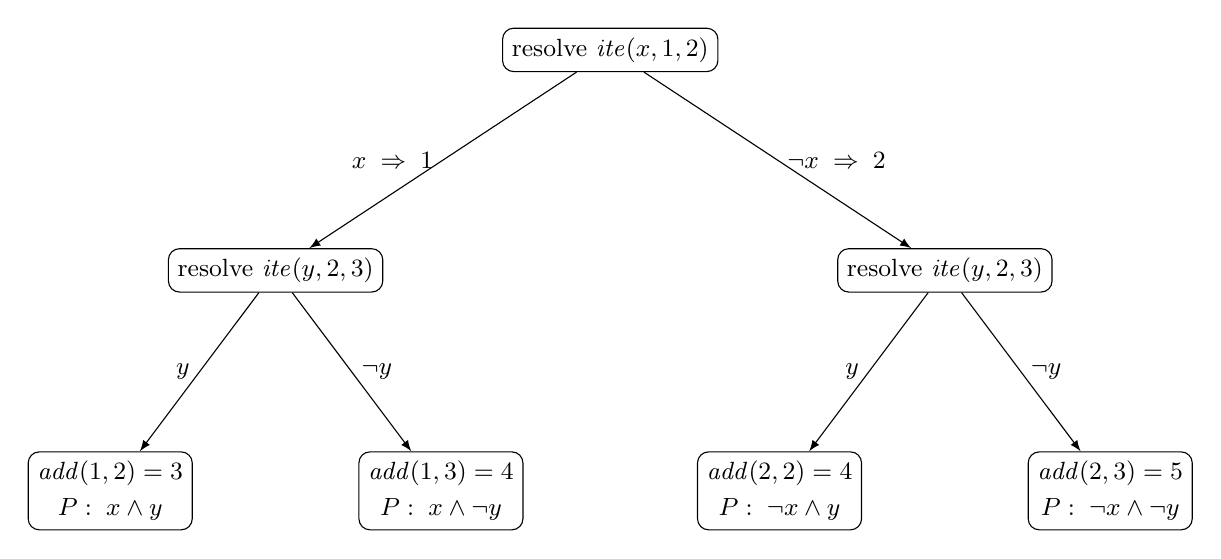
\begin{tikzpicture}[
        level 1/.style={sibling distance=8.5cm, level distance=2.8cm},
        level 2/.style={sibling distance=4.2cm, level distance=2.8cm},
        every node/.style={draw, rounded corners, align=center, font=\small},
        edge from parent/.style={draw, -latex}
    ]
    \node {resolve $\mathit{ite}(x,1,2)$}
        child { node {resolve $\mathit{ite}(y,2,3)$}
            child { node {$\mathit{add}(1,2)=3$\\[2pt]$P:\; x \land y$}
                edge from parent node[left, draw=none] {$y$}
            }
            child { node {$\mathit{add}(1,3)=4$\\[2pt]$P:\; x \land \lnot y$}
                edge from parent node[right, draw=none] {$\lnot y$}
            }
            edge from parent node[left, draw=none] {$x \;\Rightarrow\; 1$}
        }
        child { node {resolve $\mathit{ite}(y,2,3)$}
            child { node {$\mathit{add}(2,2)=4$\\[2pt]$P:\; \lnot x \land y$}
                edge from parent node[left, draw=none] {$y$}
            }
            child { node {$\mathit{add}(2,3)=5$\\[2pt]$P:\; \lnot x \land \lnot y$}
                edge from parent node[right, draw=none] {$\lnot y$}
            }
            edge from parent node[right, draw=none] {$\lnot x \;\Rightarrow\; 2$}
        };
    \end{tikzpicture}
    \caption{Path-exploration tree for $\mathit{add}(\mathit{ite}(x,1,2),\mathit{ite}(y,2,3))$. Each internal node shows an ITE being resolved; edges are labelled with the branch condition and its concrete value. Leaves show the fully resolved result and the accumulated path conditions $P$.}
    \label{fig:nested-ite-tree}
\end{figure}

Not every \textit{ite} expression necessarily results in a branch during symbolic execution. Consider the expression $ite(x>2, ite(x>1, 0, 1), 1)$: the condition of the inner \textit{ite} is already entailed by the outer condition, rendering one of its branches unreachable. To handle this precisely, we issue the following queries to the SMT solver:
\begin{enumerate}
    \item{$P\land c = \textit{SAT} \land P\land \lnot c = \textit{SAT}$}: The SMT solver says that both paths are feasible. In this case, we create two branching executions one with $P'=P\land c$ and one with $P'=P\land \lnot c$. 
    \item {$P\land c = \textit{SAT} \land P\land \lnot c = \textit{UNSAT}$}: The SMT solver says that the path such that $\lnot c$ is impossible. This means that given the information of $P$, $\lnot c$ is infeasible. As such, we do not need to add $\lnot c$ into the path, as the information is already recorded in the path. You can think of this as a node with one branch. It has no other choice so no branching executions are created. Consider $P=(x==10)\land (y==11), c=(x+y>12)$. There is no need to add $c$ to the execution path because the value is already included in $P$. 
    \item {$P\land c = \textit{UNSAT} \land P\land \lnot c = \textit{SAT}$}: She SMT solver says that the path such that $c$ is impossible. Similar to the previous case, we do not need to add $c$ onto the path as the information for deducing $\lnot c$ is already included in $P$. 
    \item {$P\land c = \textit{UNSAT} \land P\land \lnot c = \textit{UNSAT}$}: The result states that regardless of $c$ the execution is infeasible. This must mean that $P$ is infeasible, which means the constraints were infeasible. 
\end{enumerate} 

\subsection{Path Merging}

The current implementation of symbolic execution with just one \textit{ite} expression will double in size with each step. Consider the following state: $x:=\textit{ite}(i>0,x+1, x-1)$. Given the constraint that $i$ is an input and that $i$ is either $1$ or $0$, there is exists two branches in each step. As such within $5$ steps, the number of symbolic execution paths will be $2^5=32$. 

To counter state explosion, we imploy is path merging. In the previous example, consider the branch that the input is first $0$ then $1$ versus first $1$ then $0$. Both symbolic paths result in the same system state. As a result, we can combine the two paths with an $\land$ to prevent state explosion.

Figure~\ref{fig:path-merging} illustrates the first two steps of this example ($x_0$ is the initial value of $x$). Without merging, the four paths at step~2 are tracked separately. With merging, the two paths that reach $x=x_0$ (one via $i_1{=}0,i_2{=}1$ and one via $i_1{=}1,i_2{=}0$) are combined, reducing the live path count.

\begin{figure}[h]
\centering
\begin{tabular}{ccccc}
\hline
\textbf{Step} & \textbf{$i$ sequence} & \textbf{Value of $x$} & \textbf{Path condition} & \textbf{Merged?} \\
\hline
0 & --- & $x_0$ & $\top$ & --- \\
\hline
1 & $i_1{=}1$ & $x_0+1$ & $i_1>0$ & No \\
1 & $i_1{=}0$ & $x_0-1$ & $\lnot(i_1>0)$ & No \\
\hline
2 & $i_1{=}1,\;i_2{=}1$ & $x_0+2$ & $i_1>0 \land i_2>0$ & No \\
2 & $i_1{=}1,\;i_2{=}0$ & $x_0$   & $i_1>0 \land \lnot(i_2>0)$ & \multicolumn{1}{l}{$\}$ merged} \\
2 & $i_1{=}0,\;i_2{=}1$ & $x_0$   & $\lnot(i_1>0) \land i_2>0$ & \\
2 & $i_1{=}0,\;i_2{=}0$ & $x_0-2$ & $\lnot(i_1>0) \land \lnot(i_2>0)$ & No \\
\hline
2 (merged) & $i_1{\ne} i_2$ & $x_0$ & $(i_1>0 \land \lnot(i_2>0)) \lor (\lnot(i_1>0) \land i_2>0)$ & \checkmark \\
\hline
\end{tabular}
\caption{Path explosion and merging for $x := \mathit{ite}(i{>}0,\, x{+}1,\, x{-}1)$ over two steps. The two step-2 paths that reach $x_0$ are merge candidates; their path conditions are joined with $\lor$.}
\label{fig:path-merging}
\end{figure}



\section{Conclusion}

\bibliography{references}

\end{document}
